
\section{Classificatie met neurale netwerken}

Op een abstract niveau kunnen we zowel de lineaire als de logistische regressie als volgt omschrijven. We combineren een observatie $x$ met een set van gewogen waarden $\theta$ om een hypothetische output $h_\theta(x)$ uit te rekenen. Deze hypothese checken we met de werkelijke waarde $y$ en het verschil dat we hierbij vinden gebruiken we om de gewichten van $\theta$ aan te passen. Deze cyclus herhalen we totdat we vinden dat het verschil tussen onze hypothese en de daadwerkelijke waarde nagenoeg nul (of een binnen ons domein acceptabel minimum) is. Figuur \ref{img:perceptron} geeft dit proces schematisch weer. Dit plaatje, dat al in de jaren vijftig van de vorige eeuw is door F. Rosenblatt is ontwikkeld, staat bekend onder de naam \textit{perceptron} en vormt de basis voor \textit{artificiële neurale netwerken}. 


\begin{figure}[h]
\centering
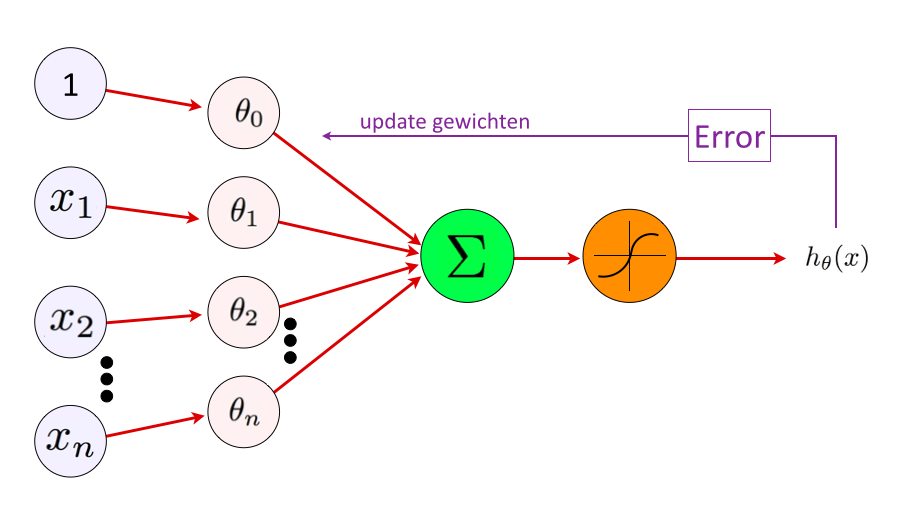
\includegraphics[width=.75\textwidth]{perceptron}
\caption{De perceptron.\label{img:perceptron}}
\end{figure}

De cirkel in figuur \ref{img:perceptron} waarin $\Sigma$ staat, kun je zien als een neuron die een getal tussen 0 en 1 teruggeeft, afhankelijk van de som van de gewogen input die deze cirkel binnenkrijgt van $x_1, x_2 \hdots, x_n$. Een neuraal netwerk bestaat uit een aantal van dergelijke neuronen (\textit{nodes}) die allemaal op basis van de gewogen som van de input een 1 of een 0 als output genereren. De perceptron in deze afbeelding zou je kunnen zien als een neuraal netwerk met $n$ \textit{input nodes} en 1 \textit{output node}.

\subsection{Forward en backpropagation}

Wanneer we het hebben over neurale netwerken, gaat het meestal over netwerken die één of meer zogenaamde \textit{verborgen lagen}(\textit{hidden layers}) hebben. Een dergelijke laag heet 'verborgen', omdat hij tussen de input- en de output-laag in zit. Elke node in de verborgen laag fungeert als een perceptron: hij is verbonden met alle nodes uit de input-laag en geeft op basis van de gewogen input een sigmoïde waarde tussen 0 en 1 door aan de volgende laag - zie figuur \ref{img:neural_net}. Wanneer een dergelijk netwerk meer dan één verborgen laag bevat, spreken we over \textit{deep learning}; het bepalen van het optimale aantal verborgen lagen en de hoeveelheid nodes per laag is onderdeel van het zogenaamde \textit{hyperparameter tuning} – een onderwerp waar we hier verder niet op in zullen gaan.

\begin{figure}[h]
\centering
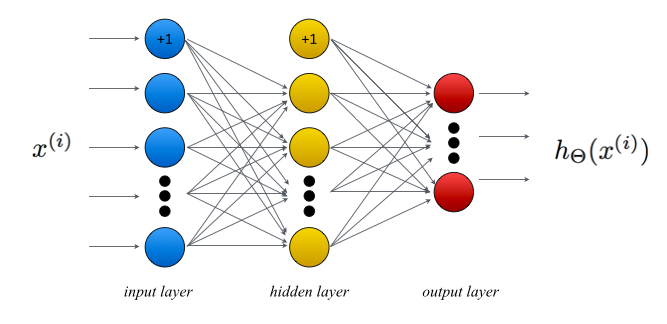
\includegraphics[width=.75\textwidth]{neural_net}
\caption{De algemene structuur van een neuraal netwerk.\label{img:neural_net}}
\end{figure}

De sigmoïde output van node $i$ in laag $l$ wordt aangeduid met $a^{(l)}_i$ (a van \textit{activation}). Omdat elke node in laag $l$ verbonden is met elke node in laag $l+1$, vormen de gewichten tussen deze nodes een matrix; deze matrix wordt aangeduid met de Griekse hoofdletter theta: $\Theta$. Het superscript van deze $\Theta$ geeft aan tussen welke lagen deze specifieke matrix geldt: de gewichten tussen de nodes in laag $l$ en laag $l+1$ zijn opgeslagen in $\Theta^{(l)}$. In het subscript wordt aangegeven tussen welke nodes in die specifieke laag dat gewicht geldt: het gewicht tussen node $i$ in laag $l$ en node $j$ in laag $l+1$ is dus weergegeven in $\Theta^{(l)}_{ji}$. 

De activatie van een specifieke node wordt bepaald aan de hand van de sigmoïdefunctie van de som van de gewogen input te berekenen. Zie figuur \ref{img:nn_example}, waarin een inputlaag van 2 nodes verbonden is met een verborgen laag van eveneens 2 nodes. Wanneer we de sigmoïdefunctie van $z$ definiëren als $g(z)$, dan is de activatie (of output) van de tweede node in de tweede laag

\[
a^{(2)}_2 = g(\Theta^{(1)}_{21} \cdot a^{(1)}_1 + \Theta^{(1)}_{22} \cdot a^{(1)}_2).
\]

\begin{figure}[h]
\centering
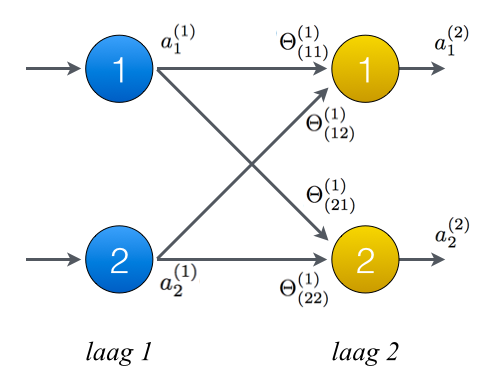
\includegraphics[width=.5\textwidth]{nn_example}
\caption{De berekening van de activatie van een node.\label{img:nn_example}}
\end{figure}

De classificatie van de input-data wordt dan bepaald door welke node in de output-laag het hoogste resultaat heeft voor deze specifieke input. Stel je bijvoorbeeld voor dat je een neuraal netwerk wilt trainen om e-mails te kunnen classificeren als spam, werk-gerelateerd, privé of familieperikelen. In dat geval zou de output-laag van het netwerk bestaan uit vier nodes, die elk één van deze categorieën representeert. Wanneer nu blijkt dat de eerste node de hoogste waarde van deze vier heeft wanneer we het netwerk een bepaalde e-mail als input geven, classificeren we deze email als spam. Om een dergelijk netwerk te kunnen trainen, hebben we dus trainingsdata nodig waarbij de input bestaat uit een zooi e-mails (platte tekst bijvoorbeeld) en de output bestaat uit een $4 \times 1$ kolomvector die voor al deze e-mails aangeeft tot welke categorie elke e-mail behoort.

De algemene werking van een neuraal netwerk kan dan in drie stappen worden samengevat:

\begin{enumerate}
\item
We gebruiken de trainingsdata als input voor het neurale netwerk. Aan de hand van deze data $x^{(i)}$ wordt op de manier die hierboven beschreven is de uiteindelijke output van het netwerk berekend. Deze stap staat bekend onder de term \textit{forward propagation}.

\item
Deze output wordt vergeleken met de verwachte waarde bij die specifieke input (de waarde van $y^{(i)}$) waardoor de we fout $\delta^{(i)}$ kunnen berekenen.

\item
Nu draaien we de richting van het netwerk als het ware om; we sturen de $\delta$ terug het netwerk in (van de de output-laag naar de eerste laag) en passen de individuele gewichten tussen de lagen op basis hiervan aan. Deze stap heet \textit{backpropagation}.

\end{enumerate}

Een cyclus van \textit{forward} en \textit{backpropagation} van alle trainingsdata wordt een \textit{epoche} (Engels: \textit{epoch}) genoemd. In de regel wordt de gehele dataset opgedeeld in kleinere \textit{batches}, en worden de gewichten aangepast nadat de foutmarge van zo'n hele batch is berekend. Het doorlopen van één batch heet een \textit{iteratie} (Engels: \textit{iteration}). Dus als je trainingsdata bestaat uit 10 datapunten en je een batch-grootte hebt van 2, dan heb je 5 iteraties nodig voor een epoche. De vraag naar verhouding tussen de batch-grootte en het aantal iteraties per epoche heeft vooral te maken met de leersnelheid en de hoeveelheid verbruikt geheugen; ook dit is weer onderdeel van de \textit{hyperparameter tuning}.


\subsection{De kostenfunctie van neurale netwerken}
Het idee van een neuraal netwerk is dat de foutmarge na een aantal epochen dusdanig klein is geworden dat we het kunnen gebruiken om een voorspelling te doen over de classificatie van \textit{nieuwe} data. Voor het berekenen van de fout van het volledige netwerk maken we opnieuw gebruik van de kostenfunctie. Omdat we nu niet te maken hebben met één enkele output (wat bij binaire classificatie wel het geval is), moeten we het totaal berekenen van alle nodes in de output-laag. Voor elke node $k$ in de output-laag gebruiken we de formule van de logistische regressie. Als we in deze laag $K$ nodes hebben (dus we willen de data classificeren in één van $K$ categorieën), dan is de kost die een voorspelling heeft met huidige waarden van $\Theta$ gegeven door 

\[
J(\Theta) = -\frac{1}{m}\left[\sum_{k=1}^m\sum_{j=1}^K 
  y_k^{(i)}log(h_\Theta(x^{(i)}))_k +
  (1-y_k^{(i)})log(1-(h_\Theta(x^{(i)}))_k) \right].
\]

Wanneer we nu één voorbeeld $(x,y)$ nemen om de $h_\Theta(x)$ in figuur \ref{img:nn_berekening} uit te rekenen, gebruiken we voor de \textit{forward propagation} het volgende stappenplan:

\begin{enumerate}
\item $a^{(1)} = x$
\item voeg toe: $a_0^{(1)} = 1$
\item bereken: $z^{(2)} = \Theta^{(1)}\cdot a^{(1)}$
\item bereken: $a^{(2)} = g(z^{(2)})$
\item voeg toe: $a_0^{(2)}=1$
\item bereken: $z^{(3)} = \Theta^{(2)}\cdot a^{(2)}$
\item bereken: $a^{(3)} = g(z^{(3)}) = h_\Theta(x)$
\end{enumerate}

\begin{figure}[h]
\centering
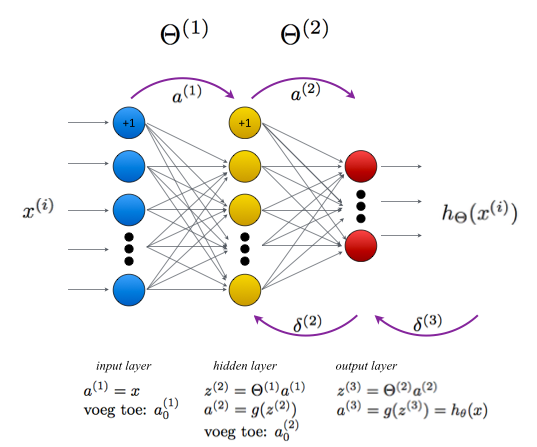
\includegraphics[width=.75\textwidth]{nn_berekening}
\caption{Het stappenplan van forward propagation.\label{img:nn_berekening}}
\end{figure}

Deze $h_\Theta(x)$ gebruiken we dan om $J(\Theta)$ uit te rekenen (onthoud dat $h_\Theta(x)$ een $K \times 1$ kolomvector is). Aan de hand van de rijvector $y$, kunnen we de foutmarge in de output-laag berekenen. Deze foutmarge gebruiken we om de fout van de \textit{individuele} gewichten in de matrices $\Theta^{(2)}$ en $\Theta^{(1)}$ te berekenen (let op dat we hier te maken hebben met een \textit{scalaire} waarde, dus de operaties op de matrices is \textit{element wise}). Het stappenplan voor de \textit{backpropagation} is dan als volgt:

\begin{enumerate}
\item bereken: $\delta^{(3)} = a^{(3)} - y$
\item bereken: $\delta^{(2)} = \Theta{(2)} \cdot \delta^{(3)} \times (g'(z^{(2)})$ (\textit{element wise})
\item update: $\Theta^{(2)} := \Theta^{(2)} + a^{(2)} \cdot \delta{(3)}$
\item update: $\Theta^{(1)} := \Theta^{(1)} + a^{(1)} \cdot \delta{(2)}$
\end{enumerate}


